% Options for packages loaded elsewhere
\PassOptionsToPackage{unicode}{hyperref}
\PassOptionsToPackage{hyphens}{url}
\PassOptionsToPackage{dvipsnames,svgnames*,x11names*}{xcolor}
%
\documentclass[
  8pt,
  ignorenonframetext,
  dvipsnames]{beamer}
\usepackage{pgfpages}
\setbeamertemplate{caption}[numbered]
\setbeamertemplate{caption label separator}{: }
\setbeamercolor{caption name}{fg=normal text.fg}
\beamertemplatenavigationsymbolsempty
% Prevent slide breaks in the middle of a paragraph
\widowpenalties 1 10000
\raggedbottom
\setbeamertemplate{part page}{
  \centering
  \begin{beamercolorbox}[sep=16pt,center]{part title}
    \usebeamerfont{part title}\insertpart\par
  \end{beamercolorbox}
}
\setbeamertemplate{section page}{
  \centering
  \begin{beamercolorbox}[sep=12pt,center]{part title}
    \usebeamerfont{section title}\insertsection\par
  \end{beamercolorbox}
}
\setbeamertemplate{subsection page}{
  \centering
  \begin{beamercolorbox}[sep=8pt,center]{part title}
    \usebeamerfont{subsection title}\insertsubsection\par
  \end{beamercolorbox}
}
\AtBeginPart{
  \frame{\partpage}
}
\AtBeginSection{
  \ifbibliography
  \else
    \frame{\sectionpage}
  \fi
}
\AtBeginSubsection{
  \frame{\subsectionpage}
}
\usepackage{lmodern}
\usepackage{amssymb,amsmath}
\usepackage{ifxetex,ifluatex}
\ifnum 0\ifxetex 1\fi\ifluatex 1\fi=0 % if pdftex
  \usepackage[T1]{fontenc}
  \usepackage[utf8]{inputenc}
  \usepackage{textcomp} % provide euro and other symbols
\else % if luatex or xetex
  \usepackage{unicode-math}
  \defaultfontfeatures{Scale=MatchLowercase}
  \defaultfontfeatures[\rmfamily]{Ligatures=TeX,Scale=1}
\fi
% Use upquote if available, for straight quotes in verbatim environments
\IfFileExists{upquote.sty}{\usepackage{upquote}}{}
\IfFileExists{microtype.sty}{% use microtype if available
  \usepackage[]{microtype}
  \UseMicrotypeSet[protrusion]{basicmath} % disable protrusion for tt fonts
}{}
\makeatletter
\@ifundefined{KOMAClassName}{% if non-KOMA class
  \IfFileExists{parskip.sty}{%
    \usepackage{parskip}
  }{% else
    \setlength{\parindent}{0pt}
    \setlength{\parskip}{6pt plus 2pt minus 1pt}}
}{% if KOMA class
  \KOMAoptions{parskip=half}}
\makeatother
\usepackage{xcolor}
\IfFileExists{xurl.sty}{\usepackage{xurl}}{} % add URL line breaks if available
\IfFileExists{bookmark.sty}{\usepackage{bookmark}}{\usepackage{hyperref}}
\hypersetup{
  pdftitle={Upward Bound},
  pdfauthor={Karina Salazar, PhD},
  colorlinks=true,
  linkcolor=Maroon,
  filecolor=Maroon,
  citecolor=Blue,
  urlcolor=blue,
  pdfcreator={LaTeX via pandoc}}
\urlstyle{same} % disable monospaced font for URLs
\newif\ifbibliography
\usepackage{graphicx,grffile}
\makeatletter
\def\maxwidth{\ifdim\Gin@nat@width>\linewidth\linewidth\else\Gin@nat@width\fi}
\def\maxheight{\ifdim\Gin@nat@height>\textheight\textheight\else\Gin@nat@height\fi}
\makeatother
% Scale images if necessary, so that they will not overflow the page
% margins by default, and it is still possible to overwrite the defaults
% using explicit options in \includegraphics[width, height, ...]{}
\setkeys{Gin}{width=\maxwidth,height=\maxheight,keepaspectratio}
% Set default figure placement to htbp
\makeatletter
\def\fps@figure{htbp}
\makeatother
\setlength{\emergencystretch}{3em} % prevent overfull lines
\providecommand{\tightlist}{%
  \setlength{\itemsep}{0pt}\setlength{\parskip}{0pt}}
\setcounter{secnumdepth}{-\maxdimen} % remove section numbering

%packages
\usepackage{graphicx}
\usepackage{rotating}
\usepackage{hyperref}

\usepackage{tikz} % used for text highlighting, amongst others
\usepackage{comment}

%title slide stuff
%\institute{Department of Education}
%\title{Managing and Manipulating Data Using R}

%
\setbeamertemplate{navigation symbols}{} % get rid of navigation icons:
\setbeamertemplate{footline}[page number]

%\setbeamertemplate{frametitle}{\thesection \hspace{0.2cm} \insertframetitle}
\setbeamertemplate{section in toc}[sections numbered]
%\setbeamertemplate{subsection in toc}[subsections numbered]
\setbeamertemplate{subsection in toc}{%
  \leavevmode\leftskip=3.2em\color{gray}\rlap{\hskip-2em\inserttocsectionnumber.\inserttocsubsectionnumber}\inserttocsubsection\par
}

%define colors
%\definecolor{uva_orange}{RGB}{216,141,42} % UVa orange (Rotunda orange)
\definecolor{mygray}{rgb}{0.95, 0.95, 0.95} % for highlighted text
	% grey is equal parts red, green, blue. higher values >> lighter grey
	%\definecolor{lightgraybo}{rgb}{0.83, 0.83, 0.83}

% new commands

%highlight text with very light grey
\newcommand*{\hlg}[1]{%
	\tikz[baseline=(X.base)] \node[rectangle, fill=mygray] (X) {#1};%
}
%, inner sep=0.3mm
%highlight text with very light grey and use font associated with code
\newcommand*{\hlgc}[1]{\texttt{\hlg{#1}}}

%modifying back ticks to add grey background
\let\OldTexttt\texttt
\renewcommand{\texttt}[1]{\OldTexttt{\hlg{#1}}}


\begin{comment}

% Font
\usepackage[defaultfam,light,tabular,lining]{montserrat}
\usepackage[T1]{fontenc}
\renewcommand*\oldstylenums[1]{{\fontfamily{Montserrat-TOsF}\selectfont #1}}

% Change color of boldface text to darkgray
\renewcommand{\textbf}[1]{{\color{darkgray}\bfseries\fontfamily{Montserrat-TOsF}#1}}

% Bullet points
\setbeamertemplate{itemize item}{\color{BlueViolet}$\circ$}
\setbeamertemplate{itemize subitem}{\color{BrickRed}$\triangleright$}
\setbeamertemplate{itemize subsubitem}{$-$}

% Reduce space before lists
%\addtobeamertemplate{itemize/enumerate body begin}{}{\vspace*{-8pt}}

\let\olditem\item
\renewcommand{\item}{%
  \olditem\vspace{4pt}
}

% decreasing space before and after level-2 bullet block
%\addtobeamertemplate{itemize/enumerate subbody begin}{}{\vspace*{-3pt}}
%\addtobeamertemplate{itemize/enumerate subbody end}{}{\vspace*{-3pt}}

% decreasing space before and after level-3 bullet block
%\addtobeamertemplate{itemize/enumerate subsubbody begin}{}{\vspace*{-2pt}}
%\addtobeamertemplate{itemize/enumerate subsubbody end}{}{\vspace*{-2pt}}

%Section numbering
\setbeamertemplate{section page}{%
    \begingroup
        \begin{beamercolorbox}[sep=10pt,center,rounded=true,shadow=true]{section title}
        \usebeamerfont{section title}\thesection~\insertsection\par
        \end{beamercolorbox}
    \endgroup
}

\setbeamertemplate{subsection page}{%
    \begingroup
        \begin{beamercolorbox}[sep=6pt,center,rounded=true,shadow=true]{subsection title}
        \usebeamerfont{subsection title}\thesection.\thesubsection~\insertsubsection\par
        \end{beamercolorbox}
    \endgroup
}

\end{comment}

\title{Upward Bound}
\subtitle{Introduction to Statistics and Enrollment Management Research}
\author{Karina Salazar, PhD}
\date{Assistant Professor, University of Arizona}

\begin{document}
\frame{\titlepage}

\begin{frame}
  \tableofcontents[hideallsubsections]
\end{frame}
\hypertarget{statistics-101}{%
\section{Statistics 101}\label{statistics-101}}

\begin{frame}{What is ``Statistics''?}
\protect\hypertarget{what-is-statistics}{}

\textbf{Statistics}: Often considered the science of uncertainty!

\medskip

The goal of statistics is to convert data (or samples!) into information
that is usable to people!

\begin{itemize}
\tightlist
\item
  Weather forecasting
\item
  Emergency preparedness
\item
  Predicting disease outbreak
\item
  Political voting polls
\end{itemize}

\medskip

Education Research:

\begin{itemize}
\tightlist
\item
  Do smaller classes improve learning?
\item
  Does offering students financial increase college completion?
\item
  Is online instruction as effective as in-class instruction?
\end{itemize}

\end{frame}

\begin{frame}{Statistics' One Big Idea: The Normal Curve}
\protect\hypertarget{statistics-one-big-idea-the-normal-curve}{}

\textbf{The Normal Distribution or Normal Curve}: natural phenomenons
(e.g., age, height, educational attainment) tend to have a similar
distributions of values.

\begin{itemize}
\tightlist
\item
  There are a few values that are small (outliers!)
\item
  Lots of values around ``the average'' (``normal observations'')
\item
  And a few values that are large (outliers!)
\end{itemize}

Outliers: observations that deviate from the ``normal'' bell curve

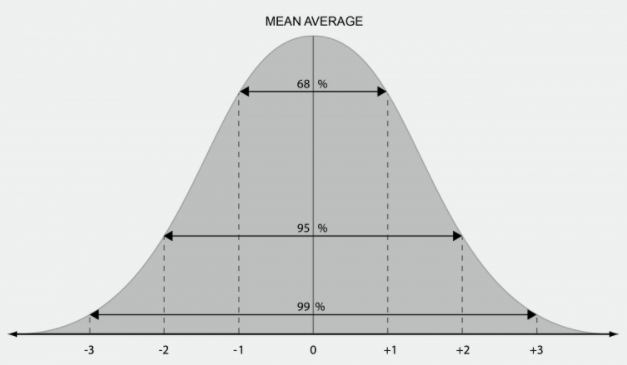
\includegraphics{normaldist.png}

\end{frame}

\begin{frame}{Statistics' One Big Idea: The Normal Curve}
\protect\hypertarget{statistics-one-big-idea-the-normal-curve-1}{}

\textbf{Women's Height in the U.S.}

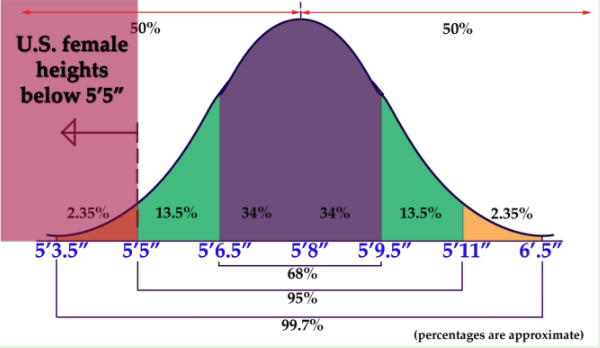
\includegraphics{women.png} \medskip

\begin{itemize}
\tightlist
\item
  BIG TAKEAWAY: There's a higher probability of data following the
  ``average'' or the ``norm''
\end{itemize}

\end{frame}

\begin{frame}{I am an outlier\ldots{} (or maybe not!)}
\protect\hypertarget{i-am-an-outlier-or-maybe-not}{}


\includegraphics{professors.png}

\end{frame}

\begin{frame}{Enrollment Management Research Program}
\protect\hypertarget{enrollment-management-research-program}{}

\begin{itemize}
\tightlist
\item
  Grew tired of mainstream access inequality policy discourse\ldots{}

  \begin{itemize}
  \tightlist
  \item
    Onus on students, families, and K-12 schools
  \item
    Enrollments can only tell us so much
  \end{itemize}
\end{itemize}

\medskip

\begin{itemize}
\tightlist
\item
  Do the enrollment management policies and practices of public
  universities undermine access for underserved student populations?

  \begin{itemize}
  \tightlist
  \item
    Universities say they care about low-income students, Students of
    Color
  \item
    But who do they actually recruit? Use data science to collect
    recruiting events!
  \end{itemize}
\end{itemize}

\medskip

\begin{itemize}
\tightlist
\item
  Policy implications

  \begin{itemize}
  \tightlist
  \item
    Too many policy decisions for increasing access attempt to ``fix''
    student behavior
  \item
    Assumption: doubling low-income, Students of Color applying to a
    university will double their enrollment
  \end{itemize}
\end{itemize}

Examples:

\begin{itemize}
\tightlist
\item
  \href{https://emraresearch.org/}{The off-campus recruiting project}
\item
  \href{https://ksalazar3.github.io/defense/\#/title}{Dissertation
  Defense}
\end{itemize}

\end{frame}

\begin{frame}{Shift The Normal Distribution!}
\protect\hypertarget{shift-the-normal-distribution}{}

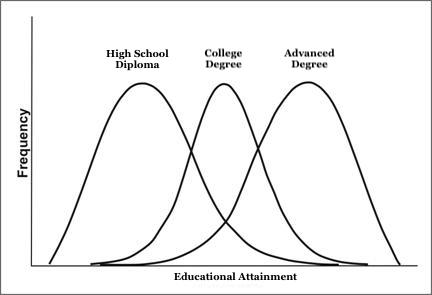
\includegraphics{shifts.jpg}

\end{frame}

\end{document}
